\section{Theoretical Analysis} \label{sec:analysis}
 


\subsection{Gain Stage}
\subsubsection{Operating Point}
The bias circuit V\textsubscript{cc}, R\textsubscript1, R\textsubscript2 will determine the base voltage V\textsubscript B and ensure the BEJ is on.

To be easier to analyse the bias circuit we can ignore the capacitors and make a Thévenin equivalent, replacing resistors R\textsubscript{1} and R\textsubscript{2}, which are in parallel, with an equivalent resistor R\textsubscript{B}:
\begin{equation}
R_B = \frac{R_{B1} R_{B2}}{R_{B1}+R_{B2}}
\end{equation}

Looking at the circuit as a voltage divider, we have
\begin{equation}
V_{eq} = \frac{R_{B2}}{R_{B1}+R_{B2}} V_{cc}
\end{equation}

To calculate the current passing through the node \textit{e} we know that I\textsubscript E =(1+$\beta_F$)I\textsubscript B.

Using the mesh analysis for the mesh on the left side and assuming that the current is going clockwise,
\begin{equation}
V_{eq} + R_B I_{B1} + V_{BEON} + R_{E1} I_{E1} = 0 \Leftrightarrow I_{B1} = \frac{V_{eq}-V_{BEON}}{R_B + (1+\beta_{FN}) R_{E1}}
\end{equation}

From this transistor model, we also know that
\begin{equation}
 I_{C1}=\beta_{FN}*I_{B1};
\end{equation}

\begin{equation}
 I_{E1}=(1+\beta_{FN})*I_{B1};
\end{equation}

\begin{equation}
 V_{c}=V_{cc}-R_{c}I_{C1};
\end{equation}

In the operating point calculations, we are also checking if the transistor is in the forward active region:  V\textsubscript{ce} = \input{../mat/FAR.tex} $>$ 0.7= V\textsubscript{BEon}, as we inteded.
\subsubsection{Incremental Analysis}
Following the operating point analysis, we can compute, the following incremental data, which concerns the bipolar transitor small signal model (AC)
\begin{align*} 
g_{m1}= I_{C1}/V_{T}\\
r_{\pi 1}=\beta_{FN}/g_{m1}\\
r_{o 1}=V_{AFN}/I_{C1}
\end{align*}

where $g_{m1}$ is the transconductance, $V_{T}$=25mV is the termal voltage, $r_{\pi 1}$ is the input incremental impedance, $\beta_{FN}$=178.7 is the common emmiter current gain, $r_{o 1}$ is the output incremental resistance, and finally, $V_{AFN}$=69.7V is the forward mode early voltage.


Assuming that the capacitor C\textsubscript{E} is a short-circuit when we are analysing the AC component, we have R\textsubscript{E}=0,

\begin{equation}
\begin{cases} 
\frac{vo}{vi}=-g_{m1} (R_C\parallel r_{o1}) \frac{r_{\pi1} \parallel R_B} {R_s+r_{\pi1}\parallel R_B} v_s \\
Z_I= R_B \parallel r_{\pi1} \\
Z_0=R_C\parallel r_{o1}
\end{cases}
\end{equation}

The results are shown in the following table.

\begin{table}[!htb]
\centering
  \begin{tabular}{|c|c|}
    \hline    
    {\bf Parameter} & {\bf Value} \\ \hline
    \input{../mat/gainstage.tex}
 \end{tabular}
 \caption{Results Gain Stage}\label{tab:gainstage}
\end{table}

As we can see, we are increasing the input voltage by 44 dB. The imput impedance is also pretty compatible with the resistance R\textsubscript S (Z\textsubscript I$>>$ ) R\textsubscript S. Unfortunately, Z\textsubscript O isn't compatible with the load impedance (8 Ohm), hence yhe inclusion of the output stage.

\subsection{Output Stage}

In this stage, we followed similar steps in order to compute the gain and impedances regarding this subcircuit.

Computing the operating point, we have

\begin{equation}
 \begin{cases}
  I_{E2}=\frac{V_{CC}-V_{EBON}-VI{2}}{R_O} \\
  I_{C2}=\frac{\beta_{FP}}{\beta_{FP}+1}I_{E2}\\
  V_{02}=V_{CC}-R_O I_{E2}
 \end{cases}
\end{equation}

Once again, we can compute, the following incremental data, which concerns the bipolar transitor small signal model (AC)
\begin{equation}
 \begin{cases}
g_{m2}= I_{C2}/V_{T}\\
r_{\pi 2}=\beta_{FP}/g_{m1}\\
r_{o 2}=V_{AFP}/I_{C2}
 \end{cases}
\end{equation}

where $g_{m2}$ is the transconductance, $r_{\pi 2}$ is the input incremental impedance, $\beta_{FP}$=227.3 is the common emmiter current gain, $r_{o 1}$ is the output incremental resistance, and finally, $V_{AFP}$=37.2V is the forward mode early voltage.

Finally, we compute the output stage's gain and impedances:
\begin{equation}
 \begin{cases}
 \frac{vo}{vi}=\frac{g_{m2}}{g_{\pi 2}+g_O+g_{o2}+g_{m2}}\\
  Z_{I2}=\frac{g_{\pi 2}+g_O+g_{o2}+g_{m2}}{g_{\pi 2}(g_O+g_{o2}+g_{m2})}\\
  Z_{02}=\frac{1}{g_{\pi 2}+g_O+g_{o2}+g_{m2}}
 \end{cases}
\end{equation}

where $g_{\pi 2}$ is the input incremental conductance, $g_{o 2}$ and $g_O$ is the $R_O$'s conductance


The results are shown in the following table.

\begin{table}[!htb]
\centering
  \begin{tabular}{|c|c|}
    \hline    
    {\bf Parameter} & {\bf Value} \\ \hline
    \input{../mat/outputstage.tex}
 \end{tabular}
 \caption{Results Output Stage}\label{tab:outputstage}
\end{table}

As we can see, $Z_{I2}$ is very compatible with gain stage's output impedance ($Z_{I2}>>Z_{01}$), hence the two subcircuits can be connected without significant loss. Also, $Z_{O2}<<R_{load}$, hence there's less amplification loss.


The theoretical operating point analysis is mostly in tune with the simulated result, for the gain stage only parameters there is a fine tune. Deviations start to occur when we compared values that are majorly influenced by the coupling of the two stages. But even then they are approximately equal.

\begin{table}[!htb]
  \begin{minipage}{.5\linewidth}
     \centering
  \begin{tabular}{|c|c|}
    \hline    
    {\bf Parameter} & {\bf Value} \\ \hline
    \input{../mat/OP.tex}
 \end{tabular}
 \caption{Results of theoretical analysis (operating point in volts)}
 \label{tab:merit}
  \end{minipage}%
    \hspace{2 mm}
    \begin{minipage}{.5\linewidth}
      \centering
        \begin{tabular}{|c|c|}
    \hline    
    {\bf Parameter} & {\bf Value} \\ \hline
    @va[i] & 1.259429e+00\\ \hline
@hvc[i] & -1.33726e+00\\ \hline
@gib[i] & -1.20692e+00\\ \hline
@id[current] & 1.009703e+00\\ \hline
@r1[i] & -1.25943e+00\\ \hline
@r2[i] & -1.20692e+00\\ \hline
@r3[i] & -5.25053e-02\\ \hline
@r4[i] & 9.318730e-01\\ \hline
@r5[i] & 2.216626e+00\\ \hline
@r6[i] & -3.27556e-01\\ \hline
@r7[i] & -3.27556e-01\\ \hline
v(1) & 1.293920e+00\\ \hline
v(2) & 3.748740e+00\\ \hline
v(3) & 5.189374e+00\\ \hline
v(3b) & 5.189374e+00\\ \hline
v(4) & 1.458724e+00\\ \hline
v(5) & -5.34994e+00\\ \hline
v(6) & 4.516972e+00\\ \hline
v(7) & 4.185212e+00\\ \hline

 \end{tabular}
        \caption{Results of simulation analysis (operating point in volts)}
        \label{compmerit}
    \end{minipage} 
\end{table}
\newpage
\subsection{Frequency Response}
 In this subsection, we tried to study the circuit's response over different input frequencies. To achieve a better high cut off frequency, we considered a transistor incremental model with capacitance, as we can see in the picture bellow.
 
 \begin{figure}[h] \centering
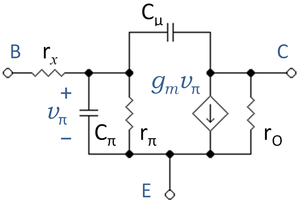
\includegraphics[width=0.4\linewidth]{transistor.png}
\vspace{-3mm}
\caption{Transistor incremental model with capacitance}\label{fig:rc}
\end{figure}

The transistors' capacitances are conccuring with the spice model.

\begin{equation}
 \begin{cases}
  C_{\pi 1}=16.1pF\\
  C_{\mu 1}=4.388pF\\
  C_{\pi 2}=14pF\\
  C_{\mu 2}=11.13pF
 \end{cases}
\end{equation}

where $C_{\pi}$ refers to the base-emitter junction capacitance and $C_{\mu}$ is the colector-base junction capacitance.

The results are the following, after loops of mesh analysis of the entire circuit:

 \begin{figure}[h] \centering
\includegraphics[width=0.5\linewidth]{frequencyresponse.eps}
\vspace{-5mm}
\caption{Theoretical Frequency Response}\label{fig:rc}
\end{figure}


\newpage
